Tous les codes de cette leçon sont dans le projet "raytracing" qui est basé sur les codes fournis sur moodle. 

\begin{figure}[H]
	\caption{\label{9_structure} Diagramme de la structure de raytracing}
	\centering
	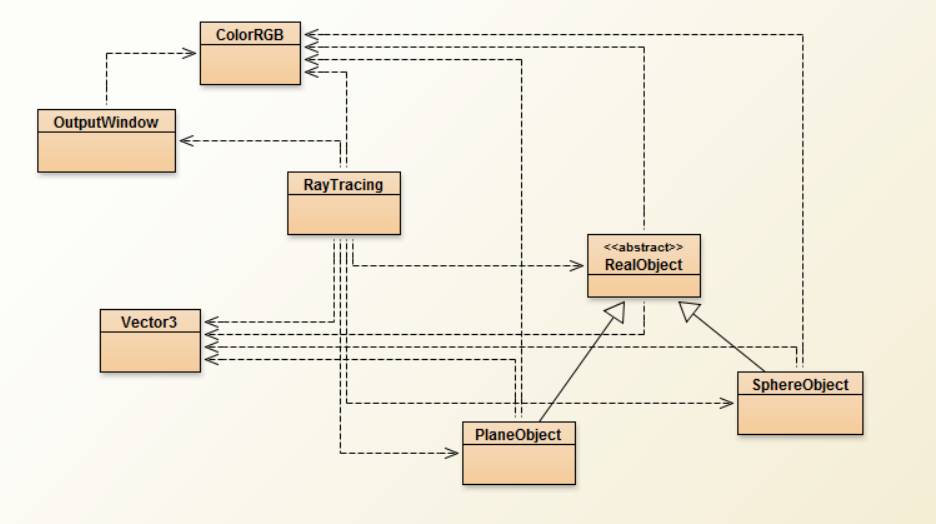
\includegraphics[scale = 0.4]{9_structure.png}
\end{figure}

\subsection{Question 1}

\subsubsection{Vector3}

Il y a dans cette classe quelques méthodes en plus de ce qui est demandé dans l'énoncé. Il s'agit de méthodes qui se sont révélées utiles par la suite lors de l'implémentation des autres méthodes.

\code{raytracing}{Vector3.java}

\subsubsection{ColorRGB}

Ici aussi, quelques méthodes complémentaires, qui seront utiles par la suite, ont été implémentées.

\code{raytracing}{ColorRGB.java}

\subsubsection{PlaneObject}
\code{raytracing}{PlaneObject.java}

\subsubsection{SphereObject}
\code{raytracing}{SphereObject.java}

\subsubsection{RayTracing}

La classe \texttt{RealObject} a du être adaptée pour que la couleur soit de type \texttt{ColorRGB} et non pas un \texttt{Vector3}.

\code{raytracing}{RayTracing.java}


\subsection{Question 2}

// TO DO

\subsection{Question 3}

Le code a directement été implementé. Il s'agit des deux denirères lignes de la méthode \texttt{traceRay} dans la classe \texttt{RayTracing}

\begin{lstlisting}
double distanceFactor = 120/Math.pow(tret, 2);
return ColorRGB.multiply(objectColor, distanceFactor);
\end{lstlisting}

\begin{figure}[H]
	\caption{\label{9_resultat} Résultat obtenu}
	\centering
	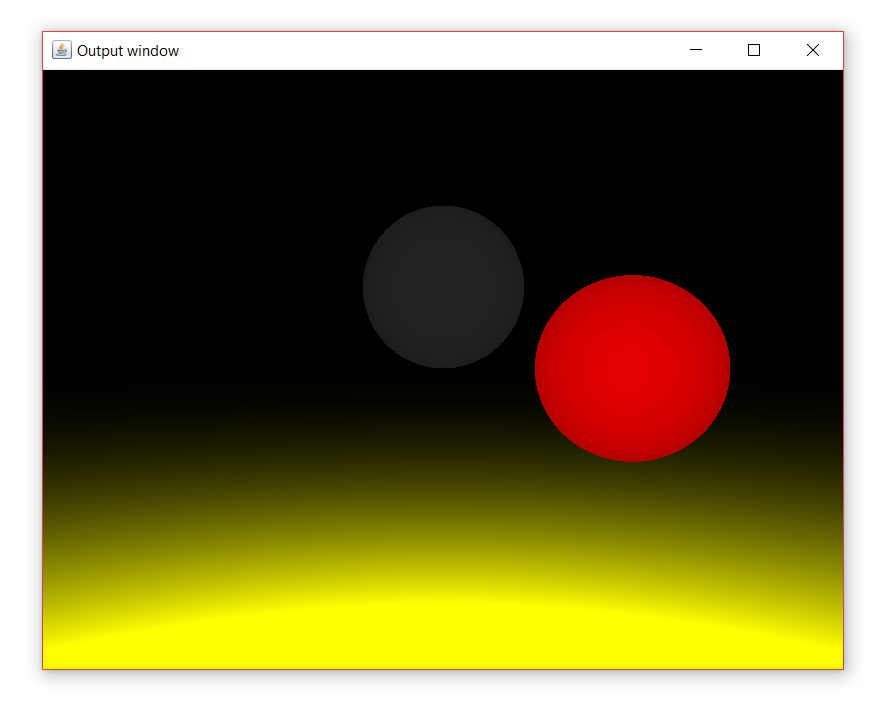
\includegraphics[scale = 0.4]{9_resultat.png}
\end{figure}